%!TEX TS-program = xelatex
\documentclass[a4paper, 12pt]{article}
\usepackage{barinovxesimple}
\renewcommand{\headrulewidth}{0.5pt} % Если необходимо убрать линейку,
\geometry{top=25mm}
\geometry{bottom=35mm}
\geometry{left=35mm}
\geometry{right=20mm}
\begin{document}
\thispagestyle{empty}
\begin{center}
    \textit{Федеральное государственное автономное образовательное\\ учреждение высшего образования }

    \vspace{0.5ex}

        \textbf{«Московский физико-технический институт\\ (национальный исследовательский университет)»}
\end{center}

\vspace{10ex}

\begin{center}
    \vspace{13ex}

    \so{\textbf{Лабораторная работа №-.-.-}}

    \vspace{1ex}

    по курсу общей физики

    на тему:

    \textbf{\textit{<<>>}}

    \vspace{30ex}

    \begin{flushright}
        \noindent
        \textit{Работу выполнил:}\\  
        \textit{Баринов Леонид \\(группа Б02-827)}
    \end{flushright}
    \vfill
    Долгопрудный \\2019
\newpage
\setcounter{page}{1}
\fancyhead[R]{\nouppercase{\leftmark}}	
\end{center}

\section{Аннотация}
В работе будут определен углы синхронизма в кристалле ниобата лития.
Будет проведено исследование зависимости генерации второй гармоники от
поляризации падающего излучения и получена экспериментальная
зависимость интенсивности генерации второй гармоники в исследуемом
кристалле от угла $\Delta \theta = \theta - \theta _{0}$ между
направлениями излучения $0$ и направлением синхронизма $\theta
_{\text{с}}$. 




\section{Теоретические сведения}

\subsection{Нелинейная оптика}

В рамках классического подхода линейность материальных уравнений и
уравнений Максвелла означала, что световые волны с разными
характеристиками распространяются в среде независимо друг от друга,
т.е. выполняется принцип суперпозиции световых волн.

При распространении мощного светового пучка через среду оптические
характеристики среды становятся зависимыми от напряженности поля
световой волны и материальное уравнение для связи поляризации среды
$\vec{P}$ с напряженностью электрического поля световой волны
$\vec{E}$ следует рассматривать в виде 
\begin{equation}
    P_i = \sum\limits_{k} \alpha _{ik}(\vec{E}) E_k
    \label{eq:1}
\end{equation}
где $\alpha _{ik}(\vec{E})$ --- компоненты тензора восприимчивости.

Тензор восприимчивости $\alpha _{ik}(\vec{E})$ в первом приближении
можно представить в виде 
\begin{equation}
    \alpha _{ik}(\vec{E}) \approx \alpha
    _{ik} + \sum\limits_{j}
    \alpha _{ikj} E_j
    \label{eq:2}
\end{equation}
Здесь $\alpha _{ik}$ --- компоненты тензора \emph{линейной
восприимчивости}, $\alpha _{ijk}$ --- компоненты тензора
\emph{нелинейной восприимчивости}.

Тогда материальное уравнение \eqref{eq:1} примет вид:
\begin{equation}
    P _{i} = \sum\limits_{k} \alpha _{ik} E_k +
    \sum\limits_{k}\sum\limits_{j} \alpha _{ikj} E_k E_j
    \label{eq:3}
\end{equation}


\subsection{Генерация второй гармоники (ГВГ)}
Пусть на среду в направлении оси $z$ падает плоская монохроматическая
волна вида
\begin{equation}
    \vec{E}(z, t) = \vec{E} ^{\omega} \cos (\omega t - k_1 z),
    \label{eq:4}
\end{equation}
где $\vec{k}_{1}$ --- волновой вектор, $k_1 = n \frac{\omega}{c}$ его компонента 
вдоль оси $z$, $n(\omega)$ --- показатель преломления среды вдоль оси
$z$ на частоте $\omega$.

Под действием световой волны в среде возникает волна поляризации с
компонентами 
\begin{equation}
    \begin{aligned}
        P _{i}(z, t) &= \sum\limits_{k} \alpha _{ik} E _{k}^{\omega}
        \cos (\omega t - k_1 z) + \sum\limits_{k}\sum\limits_{j}
        \alpha _{ikj} E _{j} ^{\omega} E _{k} ^{\omega} \cos ^{2}
        (\omega t - k_1 z) =\\
        &= \underbrace{\sum\limits_{k} \alpha _{ik} E _{k}^{\omega}
        \cos (\omega t - k_1 z)}_{\text{лин. поляризация}} +
        \underbrace{\frac{1}{2}
        \sum\limits_{k}\sum\limits_{j} \alpha _{ikj} E _{j} ^{\omega}
    E _{k} ^{\omega}}_{\text{стат. поляризация}} +\\
        &+ \underbrace{\frac{1}{2} \sum\limits_{k}\sum\limits_{j} \alpha _{ikj} E
        _{j} ^{\omega} E _{k} ^{\omega} \cos \left[ 2 (\omega t - k_1
    z) \right]}_{\text{нелин. поляризация}}
    \end{aligned}
\end{equation}

Нелинейная волна поляризации 
\begin{equation}
    P'(z,t) = P ^{2\omega} \cos (2\omega t - 2 k_1 z)
    \label{}
\end{equation}
где $P ^{2\omega} = 1/2 \sum\limits_{k}\sum\limits_{j} \alpha _{ikj}
E_j^\omega E_k^\omega$, вызывает появление вторичной световой волны с
частотой $2\omega$, интенсивность которой равна
\begin{equation}
    I ^{2\omega} = \frac{2}{3 c^3} | \overline{\ddot{P}}
    |^2
    \label{}
\end{equation}

Представим переизлученную волну в виде:
\begin{equation}
    E _{1} (z,t) = E_1 ^{2\omega} \cos (2\omega t - k_2 z)
    \label{}
\end{equation}

Условие фазового синхронизма:
\begin{equation}
    n(\omega) = n (2\omega)
    \label{eq:10}
\end{equation}

В случае изотропной среды условие синхронизма можно выполнить только в
случае аномальное дисперсии на одной из частот, но тогда эта волна
будет интенсивно поглощаться средой, и эффективного пространственного
накопления ГВГ не будет.

В случае анизотропных кристаллов величина показателя преломления $n$
зависит не только от частоты $\omega$, но и от поляризации волны. 

Если двупреломление $|n_e - n_o|$ достаточно велико, то возможно
пересечение эллипсоида $n_e (2\omega)$ и сферы $n_o(\omega)$
\ffig{fig:1}. Если известны значения $n_o$ и $n_e$ для частот $\omega$
и $2\omega$ угол синхронизма легко рассчитать, пользуясь зависимостью
показателей преломления от угла распространения луча.

\begin{equation}
    \begin{gathered}
        n_o (\theta) = const\\
        n_e (\theta) = n_o \left[ 1 + \left( \frac{n_o^2}{n_e^2} - 1
        \right) \sin^2 \theta \right] ^{-1/2}
    \end{gathered}
    \label{eq:11}
\end{equation}

 
\begin{figure}[H]
    \includegraphics[width=0.4\linewidth]{1} 
    \caption{Сечения поверхностей показателя преломления: сферы для
    обыкновенной волны ($n_o$) и эллипсоида для необыкновенной волны
$(n_e)$ в одноосном отрицательном кристалле}
\label{fig:1}
\end{figure}














\section{Оборудование}
Экспериментальная установка предназначена для исследования зависимости
интенсивности второй гармоники от ориентации нелинейного кристалла.

Экспериментальная установка собрана на оптической скамье \ffig{fig:2}.


\begin{figure}[H]
    \includegraphics[width=0.8\linewidth]{2} 
    \caption{Экспериментальная установка для изучения генерации второй
    гармоники.\\ $a$ - общий вид: 1 --- приемный блок; 2 --- окно для
наблюдения; 3 --- двухкружный гониометр; 4 --- прибор ночного
видения; 5 --- соединительный блок; 6 --- поляризатор; 7 --- лазер.\\
б --- оптическая схема: 8 --- фотодиод; 9 --- блок светофильтров; 10
--- экран; 11 --- нелинейный кристалл; 12 --- поворотное зеркало; 13
--- затвор; 14 --- объектив; 15~---~электронно-оптический
преобразователь; 16 --- окуляр; 17~---~диафрагма; 18~---~поляризатор;
19 --- лазер.}
    \label{fig:2}
\end{figure}






\section{Результаты измерений и обработка результатов}
Рассчитаем угол синхронизма для кристалла $LiNbO_3$ по формуле
\eqref{eq:11}. $n_o(\omega) \hm= 2,2336$, $n_e(\omega) = 2,1540$,
$n_o(2\omega) = 2,3225$ $n_e(2\omega) = 2,2289$.
\begin{equation*}
    \begin{gathered}
    \sin \theta = \sqrt{ \frac{n_o^2(\omega) -
    n_o^2(2\omega)}{n_e^2(2\omega) - n_o^2(2\omega)} }\\
    \theta_1 \approx 77,2^\circ 
    \end{gathered}
\end{equation*}

Угол, полученный экспериментально:
\[
    \theta_2 \approx (73 \pm 1)^\circ
\]

Генерация второй гармоники наблюдается только в положении
поляризатора, при котором на кристалл падает обыкновенная волна.

Исследуем зависимость интенсивности ГВГ в исследуемом кристалле от
угла $\Delta \theta = \theta - \theta_0$.

\renewcommand{\arraystretch}{1.3}

\begin{table}[H]
\centering
\begin{tabular}{|c|c|c|c|c|c|c|c|}
\hline
$\Delta \theta,\ '$ & 0            & 10  & 20  & 30  & 40  & 50  & 60 \\ \hline
$I ^{2\omega},\ \text{усл. ед.}$   & 100 & 85  & 65  & 60  & 55  & 55
& 55 \\ \hline \hline 
$\Delta \theta,\ '$        & 40  & 0   & -10 & -20 & -30 & -40
                           \multirow{2}{*}{}    \\ \cline{1-7}
$I ^{2\omega},\ \text{усл. ед.}$    & 50  & 105 & 105 & 70  & 50  & 50
    \\ \cline{1-7}
\end{tabular}
\caption{Зависимость интенсивности $I ^{2\omega}$ от угла $\Delta
\theta$}
\end{table}


\begin{figure}[H]
    \includegraphics[width=\linewidth]{3} 
\caption{Зависимость интенсивности $I ^{2\omega}$ от угла $\Delta
\theta$}
\label{fig:3}
\end{figure}



\section{Обсуждение результатов и выводы}
В работе определен угол синхронизма в кристалле ниобата лития:
\[
    \theta_2 = (73 \pm 1)^\circ
\]

Теоретическая оценка дает результат:
\[
   \theta_1 = 77,2^\circ 
\]

Расхождения могут быть связаны с зависимостью показателя преломления
$LiNbO_3$ от температуры.


Проведено исследование зависимости генерации второй гармоники от
поляризации падающего излучения. Наблюдать генерацию второй гармоники
можно только при обыкновенной волне, так как кристалл ниобата лития
допускает синхронную генерацию типа $oo \to e$ и не допускает
генерацию двух необыкновенных волн.


Получена экспериментальная
зависимость интенсивности генерации второй гармоники в исследуемом
кристалле от угла $\Delta \theta = \theta - \theta _{0}$ между
направлениями излучения $0$ и направлением синхронизма $\theta
_{\text{с}}$ \ffig{fig:3}.

Полученный график согласуется с теоретической зависимостью:
\begin{equation*}
    \begin{gathered}
    I ^{2\omega} \propto \sinc \left( \frac{\Delta k l}{2 \pi}
    \right)\\
    \Delta k = 2 \frac{2\pi}{\lambda_0}|n(\theta, 2\omega) -
    n_o(\omega)|
    \end{gathered}
\end{equation*}

\[
\]







\end{document}
